\documentclass[12pt,a4paper]{book}

% Formato del documento
%\usepackage[papersize={210mm,297mm},inner=3.5cm,outer=2cm,top=2.5cm,bottom=2.5cm]{geometry}
%\renewcommand{\baselinestretch}{1}
%\setlength{\parskip}{8pt}

\usepackage[utf8]{inputenc}
\usepackage{amssymb}
\usepackage{amsmath}
\usepackage{graphicx}
\usepackage{tikz}
\usepackage{tkz-graph}
\usepackage{hyperref}
\usepackage[parfill]{parskip}
\usepackage{float}
\renewcommand{\chaptername}{Capítulo}
\renewcommand{\contentsname}{Índice}
\renewcommand{\bibname}{Bibliografía}
\renewcommand{\figurename}{Figura}

\definecolor{verde_oscuro}{rgb}{0.0, 0.5, 0.0}

\newtheorem{defi}{Definición}[section]
\newtheorem{prop}{Proposición}[section]
\newtheorem{propi}{Propiedades}[section]
\newtheorem{lema}{Lema}[section]
\newtheorem{tma}{Teorema}[section]
\newtheorem{cor}{Corolario}[section]
\newtheorem{nota}{Nota}[section]
\newtheorem{ejem}{Ejemplo}[section]

\hypersetup{
    colorlinks=true,
    linkcolor=blue,
    filecolor=magenta,      
    urlcolor=cyan,
    pdftitle={Overleaf Example},
    pdfpagemode=FullScreen,
    }

\urlstyle{same}

%%%%%%%ALTERNATIVA 2%%%%%%%%%%%%
\textheight=21cm
\textwidth=17cm
%\topmargin=-1cm
\oddsidemargin=0cm
\evensidemargin=0cm
\parindent=0mm
\pagestyle{plain}
%%%%%%%%%%%%%%%%%%%%%

%%%%%%%  Comando Portada  %%%%%%%%%%%
% Ajustes de geometría si la portada sigue sin caber
% \geometry{a4paper, top=1cm, bottom=1cm, left=1cm, right=1cm} 

\newcommand{\nuevaportada}[6]{
    \thispagestyle{empty}
    \begin{center}
        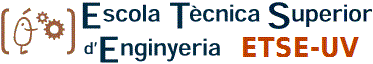
\includegraphics[width=0.5\textwidth]{images/logo.png}
        
        \vspace{0.3cm} % Espacio reducido
        {\Large\bfseries\textsc{M\'aster Universitario en #1}\par}
        
        \vspace{0.3cm} % Espacio reducido
        
\includegraphics[width=0.4\textwidth]{images/uv.png}
        
        \vspace{0.3cm} % Espacio reducido
        {\Large\bfseries\textsc{Trabajo de Fin de M\'aster}\par}
        
        \vspace{0.5cm} % Mantener este espacio un poco más grande para el título
        {\Large\bfseries #2\par}
        
        \vspace{1.5cm} % Reducido a 1.5cm desde 2cm
        \begin{flushright}
            \begin{tabular}{l} 
                {\large\bfseries\textsc{Autor:}} \\
                {\large\textsc{#3}} \\ [0.3cm] % Espacio reducido
                {\large\bfseries\textsc{Tutora:}} \\ 
                {\large\textsc{#4}} \\ [0.3cm] % Espacio reducido
                {\large\bfseries #5} 
            \end{tabular}
        \end{flushright}
    \end{center}
    % Eliminamos \clearpage de aquí, ya que la portada debe ser una sola página
    % Si necesitas un salto de página después de la portada, lo añades en el documento principal.
}

\begin{document}

\nuevaportada{Ciencia de Datos}{Problema de Localización de Centros k-Balanceado Multiobjetivo}{Manuel Rubio Martínez}{Anna Martínez Gavara}{Abril, 2025}

\clearpage

\newpage
\tableofcontents

\chapter{Preliminares}
\section{primera parte}

\begin{defi}
Un algoritmo \textbf{"greedy"} (codicioso) es un método construcción de soluciones para un problema de optimización,
de manera que en cada paso se escoge la mejor posible, aunque esto no lleve finalmente a un óptimo global.
\end{defi}

\bigskip

\begin{defi}
Un algoritmo \textbf{"greedy randomizado"} se basa en el "greedy", pero en cada paso se elige de forma aleatoria entre un conjunto de mejores opciones.
Si el conjunto de opciones es el total, el algoritmo es "random".
\end{defi}

\chapter{Introducción}

\section{Antecedentes}
\subsection{Optimización Combinatoria}

Es la rama de la optimización enfocada en encontrar óptimos en conjuntos de soluciones finitos.
Esto no significa que el problema sea fácil, al contrario, por lo general es un problema NP-complejo. \\
Que sea NP-complejo implica que conforme el número de soluciones aumenta, la complejidad computacional lo hace, a su vez, exponencialmente. \\
Un ejemplo de ello es el problema sobre el que trata este TFM, 
tratar de que encontrar, en un conjunto de $n$ elementos, un subconjunto $k$ de ellos tal que  minimice varias funciones objetivo.
\\ \\
Es rápido calcular las combinaciones posibles (siempre suponiendo $k \leq  n$) son:

$$
    \binom{n}{k} = \frac{n!}{(n-k)!k!}
$$

Por ejemplo, si $n=50$ y $k=5$, entonces
$$
    \frac{50!}{(50-5)!5!}=2118760
$$
para un problema bastante sencillo. Para casos reales, podríamos tener n=5000 y k=50, la cantidad de posibles solucones sería del orden de $2.28  e^{120}$. Contabilizando el coste de 
evaluación de cada solución, no es viable encontrar el óptimo de forma exacta. Incluso utilizando los ordenadores más potentes, estaríamos hablando de tiempos astronómicos.

\subsection{Metaheurísticos}

Las metaheurísticas aparecen con el desarrollo de las ciencias de la computación, como principal solución a estos problemas. Donde los métodos exactos no serían capaces de encontrar el óptimo,
los Metaheurísticos buscan soluciones `buenas` en tiempos de ejecución razonables, sacrificando la garantía que proporcionan los métodos exactos de obtener un óptimo global.

Generalmente combinan heurísticas para obtener soluciones buenas, con aleatoriedad, para conseguir una exploración
más ámplia del conjunto de soluciones posibles, buscando un balance entre exploración y explotación del entorno de soluciones.\\
Exploración ya que no se quedan bloqueados en regiones aisladas, intentando buscar óptimos locales, sino que recorren el resto del espacio buscando nuevas soluciones.\\
Explotación porque cuando entran en una región, profundizan en ella buscando los mejores óptimos locales.

Son algoritmos muy generales, fáciles de implementar y adaptables a casi 
cualquier problema de optimización.

Los principales metaheurísticas son:
\begin{itemize}
    \item Algoritmos Genéticos (GA - Genetic Algorithms)\\
    Inspirados en la selección natural y el funcionamiento de la genética, se basan en la generación aleatoria de soluciones, y el cruce de las más prometedoras entre sí, 
    añadiendo mutaciones. El cruce de las más prometedoras crea soluciones buenas, mientras las mutaciones aumentan la diversidad.
    \item Recocido Simulado (SA - Simulated Annealing)\\
    Basada en la física, se basa en el proceso de recocer metales (calentarlos y enfriarlos para alterar su estructura). Explora soluciones aceptando movimientos de mejora, pero también que puedan empeorar, 
    en función de una probabilidad dependiente de la "temperatura", que decrece con el paso de las iteraciones. Al principio, una temperatura alta favorece la exploración, y al final una baja favorece la explotación.
    \item Búsqueda Tabú (TS - Tabu Search)
    Genera una lista `Tabú` que actúa como memoria del algoritmo, incluyendo los movimientos recientes con el objetivo de no repetir soluciones recientes, sino explorar nuevas, aunque estas no sean las mejores posibles. Esto favorece la exploración.
    \item Optimización por Colonia de Hormigas (ACO - Ant Colony Optimization)
    Diseñado para problemas de rutas, construyendo soluciones iterativamente a través de un grafo, cuyas aristas  se van pesando a medida que generan soluciones buenas.
    %\item Optimización por Enjambre de Partículas (PSO - Particle Swarm Optimization) noo se si incluirlo
\end{itemize}


\subsection{GRASP (Greedy Randomized Adaptive Search Procedure)}
% No se si indicar, en todos los casos, que es para problemas de combinatoria

Desarrollado a finales de los años 80, se crea específicamente para resolver problemas complejos de optimización combinatoria.

El algoritmo se fundamenta en dos partes, una primera en la que se genera una solución aleatorizada, y una segunda en la que se realiza una búsqueda local.
Estos dos pasos se ejecutan múltiples veces, y la mejor solución encontrada es la que se devuelve como resultado final.

\begin{itemize}
    \item Fase de Construcción (Greedy Randomizada):
    Para problemas de combinatoria, empieza incorporando un elemento de manera aleatoria a la solución. Desppués, se crea una LRC (Lista Restringida de Candidatos) con los `mejores candidatos`. Después,
de esta lista se selecciona uno de manera aleatoria, y se añade a la solución. Se repite hasta que la solución contiene la cantidad necesaria de elementos para ser válida.
    \item Búsqueda Local:
    Se toma la solución generada en la fase de construcción, y se intenta mejorar. Se coge cada elemento de la solución, y se prueba a cambiar por alguno de los elementos aún no seleccionados para la misma. Si con alguno la solución mejora, se intercambia.
    Se sigue con el proceso hasta que no se puede mejorar más. Entonces se guarda la solución, y se vuelve a reejecutar el algoritmo completo.
\end{itemize}

Como la búsqueda local se puede hacer a partir, incluso, de otros algoritmos, al final el GRASP
es muy generalizable. También se han creado muchas otras versiones, como añadir mutaciones (como en el algoritmo genético) para, después de realizar
una búsqueda local, poder seguir.

La versión del artículo en el que me baso para comparar los resultados del GRASP que voy a diseñar utiliza \textbf{path-relinking}, que explicaré en la parte de estado del arte.




\section{Problemas de Localización}

Los \textbf{problemas de localización} son uno de los tipos principales de optimización combinatoria, que buscan determinar la ubicación óptima para construir instalaciones, como almacenes, centros de distribución, hospitales, escuelas o estaciones de bomberos. 

Algunos de los objetivos a optimizar pueden incluir la minimización de la distancia total o máxima a los clientes, la reducción del coste operacional, la maximización de la cobertura de la demanda, la mejora del tiempo de respuesta, el balance de uso entre las instalaciones etc.

Estos problemas son de vital importancia en la práctica en múltiples sectores. En la \textbf{logística} y la gestión de la cadena de suministro, la correcta ubicación de almacenes y centros de distribución puede reducir drásticamente los costes de transporte y mejorar la eficiencia de la entrega. En el ámbito de la \textbf{salud}, la localización de hospitales y clínicas asegura un acceso equitativo a la atención médica y tiempos de respuesta rápidos en caso de emergencia. Asimismo, en la planificación de \textbf{servicios públicos}, como la ubicación de escuelas o parques de bomberos, se busca garantizar la accesibilidad cobertura del total o la mayoría de la población.

Entre los ejemplos clásicos y más estudiados de problemas de localización se encuentran:

\begin{itemize}
    \item \textbf{Problema del Viajante (TSP - Traveling Salesman Problem)}: Es el clásico problema de buscar la ruta más corta que permita recorrer un conjunto de lugares exactamente una vez, y luego regresar al punto de origen. Dependiendo del contexto, la función objetivo puede ser minimizar la distancia total del viaje, el tiempo invertido, o una combinación de ambas.\\
Existen variantes donde se ha de seleccionar subconjunto de lugares, considerando, además de los factores distancia y tiempo, un peso o valor añadido dependiendo de la selección hecha.\\
Algunos de los ejemplos más tipicos de este problema es la planificación de rutas de reparto, ruta más eficiente para la recolección de residuos de una ciudad, la planificación de un viaje por por las principales atracciones turísticas de un pais etc.

    \item \textbf{Problema de Ruteo de Vehículos (VRP - Vehicle Routing Problem)}: Se trata de encontrar la mejor manera de diseñar y organizar las rutas que deberán recorrer uno o varios vehículos para realizar entregas para un conjunto de ubicaciones. Se suele buscar minimizar los tiempos de entrega, la distancia recorrida, el coste operativo, y también suelen tener restricciones 
en la capacidad de los vehículos, tiempos u horarios de entrega, tiempo máximo de la ruta etc.\\
Los ejemplos más comunes son la coordinación de camiones de reparto de pedidos, organización del transporte público con buses urbanos, también para la recolección de residuos etc.
    \item \textbf{Problemas de Localización (Facility Location Problems)}: Se busca intentar determinar cuáles son los mejores lugares para instalar varias infraestructuras (almacenes, puntos de distribución, hospitales). El objetivo, si el problema trata únicamente de construir la infraestructura, es minimizar costes/maximizar beneficios, pero generalmente existe también un grupo de clientes o usuarios a los que hay que atender desde los puntos de distribución Con esto el objetivo puede ser reducir la distancia total para suministrar, equilibrar
el uso de las infraestructuras, y también tener restricciones de demanda, de cobertura, etc.\\
Hay ejemplos como elegir dónde ubicar almacenes, ubicar estaciones de ambulancias, colocar torres te telefonía o decidir dónde abrir nuevos comercios de una cadena de supermercados.
\end{itemize}


\section{Motivación y caso práctico}

\subsection{Motivación}
En un entorno cada vez más competitivo y cambiante, la localización estratégica de infraestructuras no solo debe considerar criterios tradicionales como la distancia o el coste, sino también otros factores clave como la cobertura del mercado, la accesibilidad y el equilibrio en la distribución de la demanda.

Actualmente, uno de los principales retos es maximizar el alcance de ciertos productos o servicios, garantizando que lleguen al mayor número posible de personas. Al mismo tiempo, es necesario evitar la concentración excesiva de demanda en unos pocos puntos, lo que puede provocar saturación, pérdida de calidad del servicio o ineficiencias operativas, mientras existen centros que, por tener una localización más aislada, prácticamente no reciben demanda.

Este equilibrio entre amplitud de cobertura y uso equilibrado de los recursos disponibles es especialmente importante en contextos donde hay un reducido número de emplazamientos posibles, y donde cada selección de localización afecta tanto a la eficiencia del sistema como a la experiencia del usuario o cliente final.

Al abordar el problema es importante considerar que la distancia total o el tiempo medio de viaje no es el factor más crítico. Por ejemplo, si construyes un hospital en una ciudad, el objetivo no es que la población viva lo más cerca posible, sino que se
los residentes se encuentren a una distancia razonable. 

Considera estos dos escenarios para una ciudad:
\begin{itemize}
    \item Escenario 1: El tiempo medio de viaje a un hospital es de 15 minutos, y el tiempo máximo de viaje para cualquier individuo es de 30 minutos.
    \item Escenario 2: El tiempo medio de viaje a un hospital es de 13 minutos, pero el tiempo máximo de viaje para cualquier individuo es de 1 hora
\end{itemize} 
En tiempo global, podríamos decir que el segundo sistema implementado es más eficiente, pero se dejan de lado los valores extremos extremos. Una parte significativa de la población podría tener grandes dificultades para acceder a servicios esenciales. Por el contrario, aunque el primer caso tenga un tiempo medio mayor, mejora considerablemente la accesibilidad. Esto subraya que mejorar la media no necesariamente mejora el servicio.

\subsection{Caso práctico}
Una red hospitalaria está planificando la ubicación de 5 centros médicos dentro de una región con una población de $400$ personas. Debido a limitaciones presupuestarias, de personal e infraestructura, se restringe su construcción a un número $20$ de posibles emplazamientos. El objetivo será encontrar qué $5$ centros, de ese total de $50$ posibles, habrá que construir,teniendo en cuénta los siguientes criterios:

\begin{itemize}
    \item Cobertura Poblacional: Los centros seleccionados deben intentar minimizar la máxima distancia o tiempo de viaje entre el conjunto de la población y los centros médicos.
    \item Capacidad: Hay que intentar que los centros médicos no queden sobresaturados. Construir un único centro médico en una zona con mucha población puede generar una buena cobertura y tiempos de viaje cortos, pero quedar saturado y generar problemas de tiempo de atención y espera.
    \item Equilibrio: No queremos tampoco que haya centros médicos con poco uso, intentando que la diferencia entre los más usados y los menos sea la menor posible, con lo que el uso quede bien repartido.
\end{itemize}
Caso de ejemplo ficticio utilizando la zona de Valencia:
\begin{figure}[htbp]
    \centering
    \begin{minipage}[c]{0.45\textwidth}
        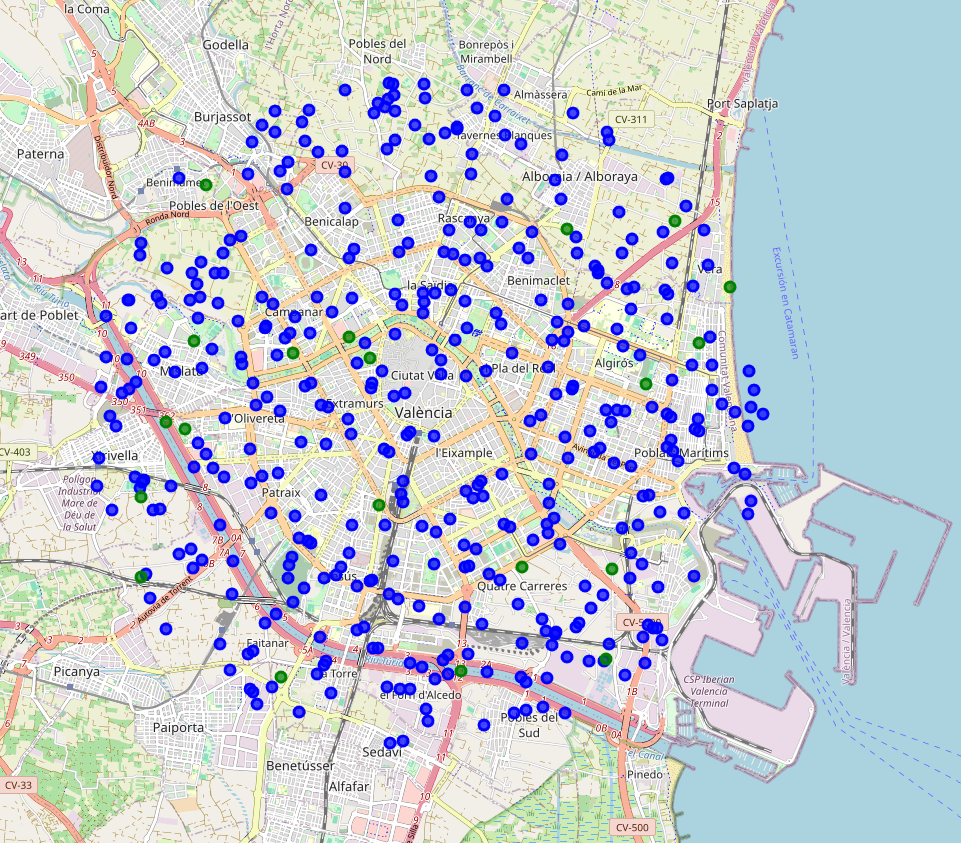
\includegraphics[width=\textwidth]{images/ejemplo_centros_medicos.png}
        \label{fig:poblacion_centros_medicos}
    \end{minipage}
    \hfill
    \begin{minipage}[c]{0.45\textwidth}

        Se representa con 400 puntos azules a la población de la ciudad y alrededores de Valencia. También con 20 puntos verdes las posibles localizaciones de los centros médicos.
    \end{minipage}
    \caption{Población y centros médicos}
\end{figure}

\begin{figure}[htbp]
    \centering
    \begin{minipage}[c]{0.45\textwidth}
        Ejemplo de solución aleatoria, escogiendo únicamente 5 centros médicos. Podemos ver que al escogerse por el sur y oeste, queda gran parte de valencia con una importante dificultad de acceso a los mismos.
    \end{minipage}
    \hfill
    \begin{minipage}[c]{0.45\textwidth}
        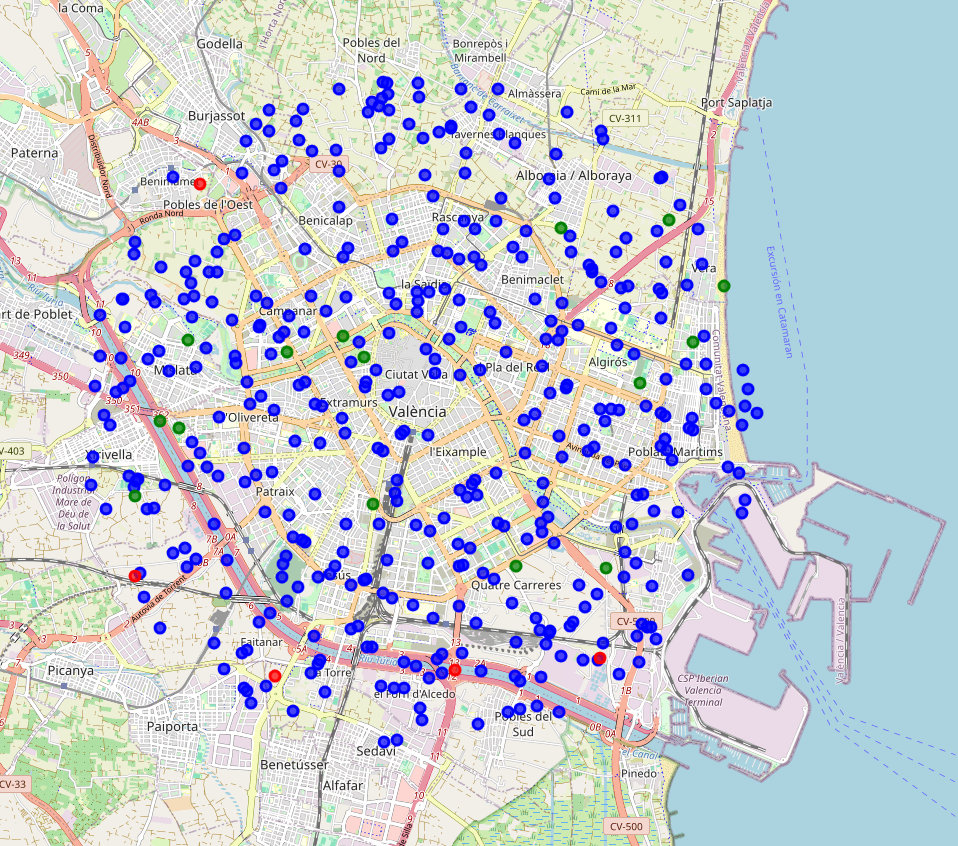
\includegraphics[width=\textwidth]{images/solucion_ejemplo_1.png}
        \label{fig:ejemplo_1}
    \end{minipage}
    \caption{Primer ejemplo de solución}
\end{figure}

\begin{figure}[htbp]
    \centering
    \begin{minipage}[c]{0.45\textwidth}
        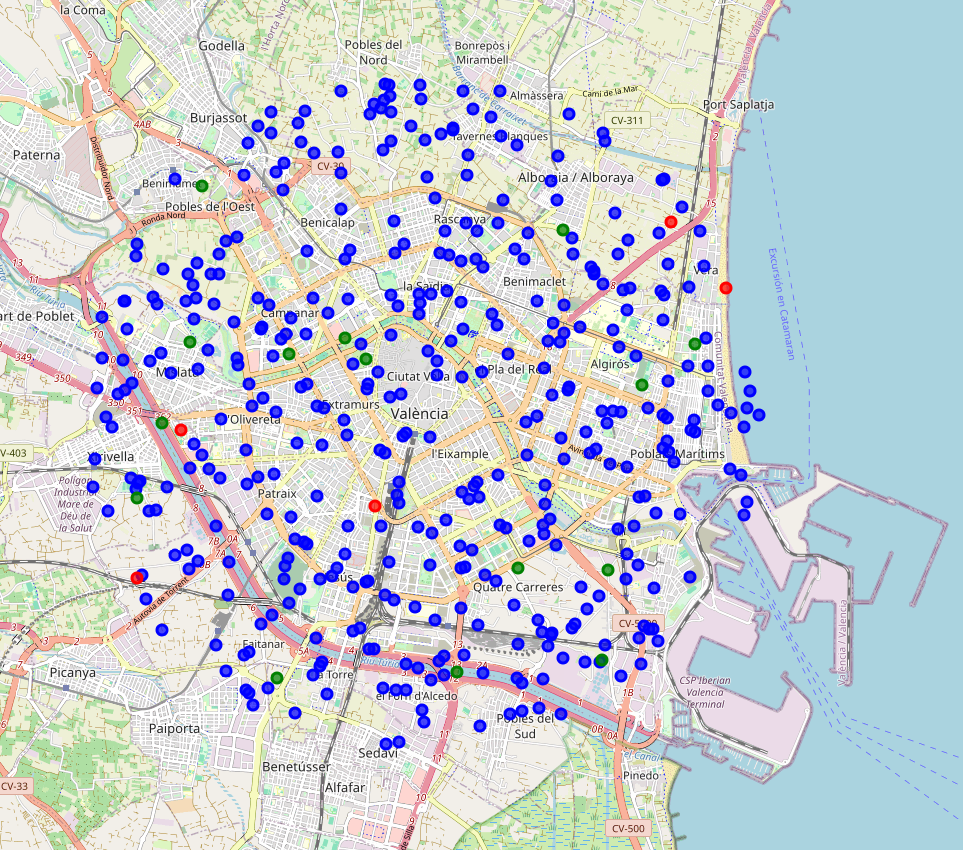
\includegraphics[width=\textwidth]{images/solucion_ejemplo_2.png}
        \label{fig:ejemplo_2}
    \end{minipage}
    \hfill
    \begin{minipage}[c]{0.45\textwidth}
        Aquí ya se pueden ver mejoras, pero sigue sin ser una buena solución. Por el sur y el norte tienen aún bastante lejos los centros médicos, y hay alguno como el de la izquierda del todo, por Valencia Sud, que se utilizará relativamente poco al ir la población a los otros 2 más centricos (estos a su vez quedarán sobre saturados).
    \end{minipage}
    \caption{Segundo ejemplo de solución}
\end{figure}

\begin{figure}[htbp]
    \centering
    \begin{minipage}[c]{0.45\textwidth}
        Esta solución sería, de las 3, la que mejor apariencia tiene, con una dispersión de los centros médicos mejor, y solo dejando más apartada la zona sur del puerto.
    \end{minipage}
    \hfill
    \begin{minipage}[c]{0.45\textwidth}
        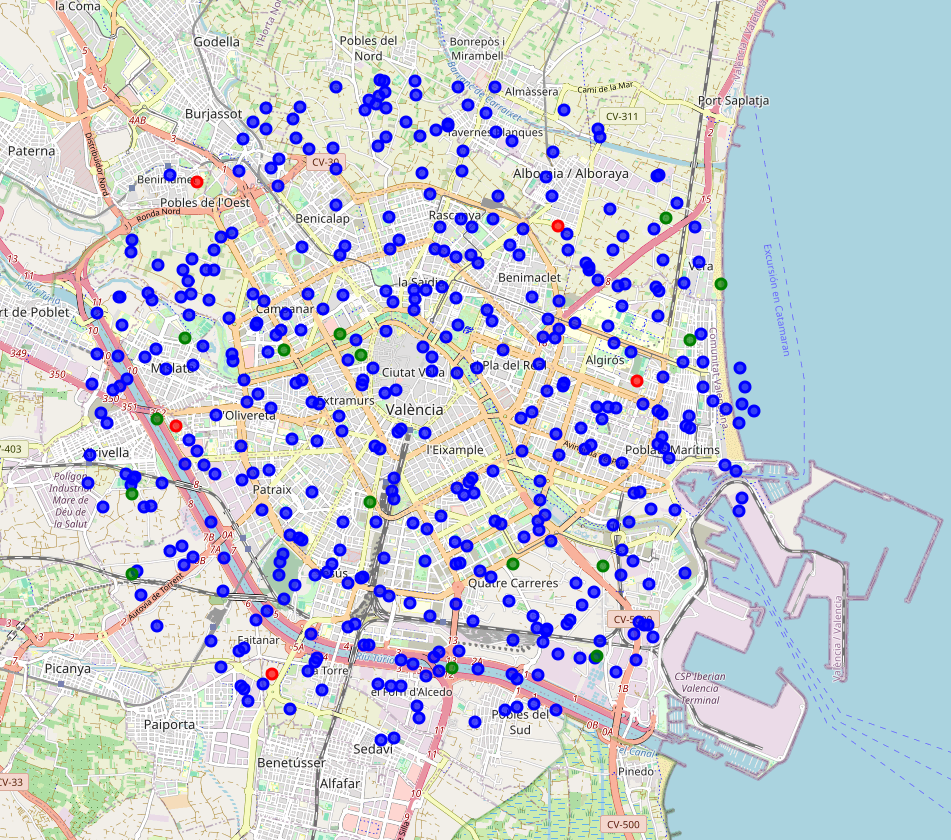
\includegraphics[width=\textwidth]{images/solucion_ejemplo_3.png}
        \label{fig:ejemplo_3}
    \end{minipage}
    \caption{Tercer ejemplo de solución}
\end{figure}

\newpage

\section{Estado del arte}

Voy a basarme en el artículo \cite{k-Balanced}



\chapter{Modelo Matemático}


\section{Definición}
3 variables a minimizar
restricciones
método exacto? (no viable)

\chapter{Implementación del Grasp}

Primera versión, grasp simple con inicialización aleatoria y búsqueda local en una de las 3 variables

Segunda versión, grasp con inicialización greedy randomizada (con alpha fijo) y 2 búsquedas locales en serie

Tercera y última versión, grasp con inicialización greedy randomizada (con alpha ranodom), búsquedas locales escogidas por aprendizaje reforzado.

\chapter{Aprendizaje Reforzado}

\chapter{Experimentación y Resultados}

Instancias, comparativa, CASO DE ESTUDIO

\chapter{Conclusiones}





\begin{thebibliography}{X}
    \bibitem{k-Balanced} \textsc{Sánchez-Oro, Jesús; López-Sánchez, Ana D.; Martínez-Gavara, Anna; Hernández-Díaz, Alfredo G.; Duarte, Abraham}. \textit{A Hybrid Strategic Oscillation with Path Relinking Algorithm for the Multiobjective k-Balanced Center Location Problem.} Mathematics, Vol. 9, No. 8, 2021, Artículo 853. \url{https://www.mdpi.com/2227-7390/9/8/853}

\end{thebibliography}


\end{document}

